% ReXGrounding Challenge paper: team method description (Appendix A)
% ---------------------------------------------------------------
% Please keep this to about half a page of text (300-450 words) plus one optional
% figure. Keep the headings below in this order; write "none" where something
% does not apply. We will typeset and may
% lightly edit for length and style. Citations: please list the reference at
% the end of the file in plain text; we will add them to the bibliography.

\subsection{fomofo (rank 3)}
\label{app:fomofo}

% Everything the model saw in training, with sizes and licences. Include the
% challenge data, public datasets, in-house data, pretrained weights, and any
% derived labels (pseudo-labels, LLM-extracted text, anatomy masks). State
% explicitly whether any test-set scans, in image or text form, were used at any
% stage, including pretraining of components you did not train yourselves.
\paragraph{Data} We trained on the challenge training (2,992 scans) and validation (200 scans) sets. External data: 8,000 CT-RATE~[9] sentence--mask pairs (nodule and effusion pseudo-masks from TotalSegmentator~[8]) for two members (one of them only the 1,540 effusion pairs). In-house: TAP-CT~[2] pretraining only (105k CT volumes). Pretrained weights: VoxTell v1.1~[1], Qwen3-Embedding~[5], TAP-CT-B-3D, Qwen2.5-7B~[7]. Derived: TotalSegmentator lobe masks, a Qwen3-32B~[6] lobe mapping of all finding sentences, synonym-based text augmentations and Qwen2.5 paraphrases (TAP-CT). Test-set exposure: the CT-RATE pool incidentally included test studies, so one member saw 80 of the 300 test studies and the other 10 of these, as image, report sentence and pseudo-mask, never challenge masks or sentences. Retraining both with these studies replaced by other CT-RATE scans changed the final masks equally on exposed and unexposed studies (Dice 0.976 vs 0.974 between versions). Licences: CT-RATE and VoxTell CC BY-NC-SA 4.0, TAP-CT CC BY-NC 4.0, Qwen Apache-2.0.

% Resampling, orientation, intensity windowing or normalisation, cropping, patch size.
\paragraph{Pre-processing} VoxTell uses the native grid, z-scored intensities and random $192^3$ crops, one third centred on a finding. TAP-CT resamples to 1.5\,mm isotropic, clips to $[-1008, 822]$\,HU and z-scores, and uses $24\times224\times224$ crops ($4\times8\times8$ ViT patches).

% Image backbone, text encoder, how the text conditions the image model, number
% of parameters if known. Name the base framework (for example VoxTell, nnU-Net).
\paragraph{Architecture and text encoder} VoxTell: an nnU-Net~[3,4] residual encoder and a transformer decoder in which the frozen Qwen3-Embedding-4B sentence embedding queries the $12^3$ bottleneck tokens (440M trainable parameters). TAP-CT is a 3D ViT-B (87M parameters) FiLM-conditioned~[10] on Qwen3-Embedding-0.6B, followed by a convolutional decoder.

% Loss, optimiser, learning-rate schedule, batch size, epochs or steps, data
% augmentation (image and text), hardware and training time, whether the
% validation set was used for training and how.
\paragraph{Training} VoxTell: deeply supervised Dice plus cross-entropy (Tversky in three members), SGD at $10^{-4}$ with polynomial decay, batch size 8. Members were trained from VoxTell v1.1 for 250 epochs, five of them for up to 430 (about 7\,h per 250 epochs on one H100). No image augmentation; text augmentation swapped phrases for equivalent phrasings seen in the data ($p=0.5$). Validation data were in every member's training set. TAP-CT: Dice plus cross-entropy, AdamW, batch size 16, 50k steps with the encoder frozen then 25k fine-tuning (4.5\,h per seed on one H100), five seeds, on training plus validation data, with left--right flips, paraphrases and location-swapped negatives.

% Number of models in the final submission, how they differ, how predictions were combined.
\paragraph{Ensembling} The probability maps of twelve VoxTell members (differing in initialisation, loss, sampling and auxiliary data) are averaged and fused 0.8/0.2 with the mean of five TAP-CT seeds (Figure~\ref{fig:tags}).

% Thresholding, component selection, anatomical restriction (lobe or side),
% any use of an LLM at inference.
\paragraph{Post-processing} The fused map is restricted to the named lobe (dilated 16 voxels) or lung (12 voxels), cut at a per-finding threshold from a gradient-boosted regressor, cleaned by a small 3D CNN that drops components predicted to lower Dice (both fitted on validation), and contested voxels go to the most confident finding. LLM at inference: only the Qwen3-32B lobe mapping.

% Average time per scan per finding at inference, and the hardware used.
\paragraph{Inference time and hardware} On one H100, a VoxTell member takes 3.7\,min per scan (stride $1/8$, all findings jointly), about 24 GPU-min per finding for twelve members; the five TAP-CT seeds together take 23\,s per scan.

% Which submission is the final one (model name as shown on the leaderboard),
% and one or two sentences on what helped most and what did not help.
\paragraph{Final submission and lessons} Our final submission is TAGS\_TAPv3 (0.362 on the full test set). Most helpful were TAP-CT as a second architecture, the dilated restriction and per-finding thresholds; changes for location words, pseudo-labels and extra public data did not help. Four late post-processing additions each gained 0.001--0.004 on validation and the public half, yet our submission without them scored 0.365 on the full set.

% Link(s) to code and weights, with licence; or state that they are not released.
\paragraph{Code and weights availability} Code: \url{https://github.com/nki-radiology/TAGS-ReXGroundingCT} (Apache-2.0). Weights of all members: \url{https://huggingface.co/fomofo/TAGS-ReXGroundingCT} (CC BY-NC-SA 4.0; TAP-CT seeds CC BY-NC 4.0).

% Optional: one figure of the architecture or pipeline (vector PDF preferred).
\begin{figure}[h]\centering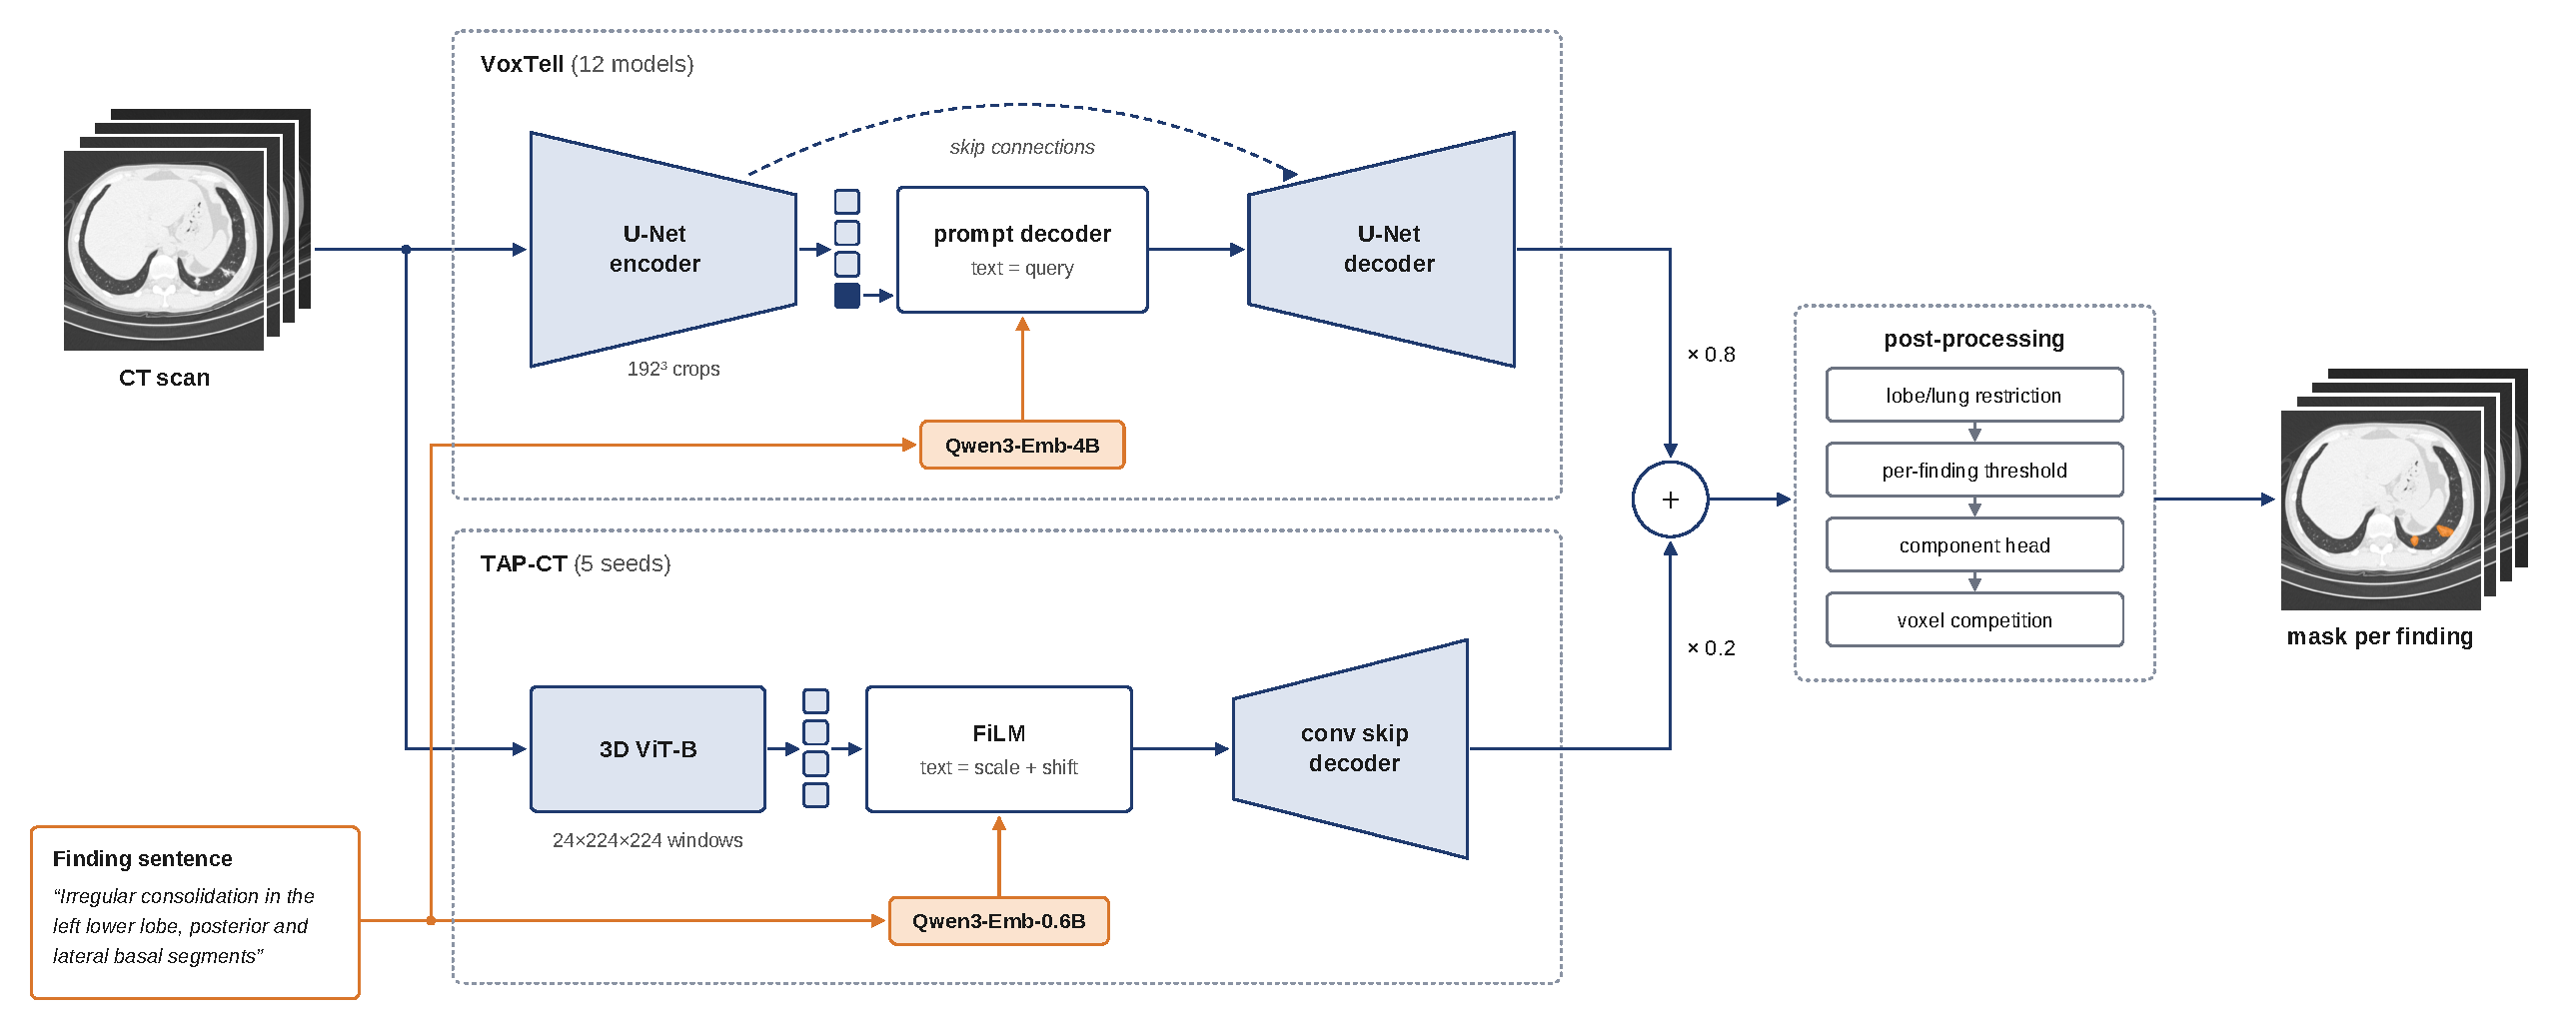
\includegraphics[width=\textwidth]{TAGS_architecture.pdf}\caption{<The TAGS pipeline: twelve VoxTell models and five TAP-CT seeds, each conditioned on the finding sentence, produce probability maps that are averaged per branch and fused 0.8/0.2, followed by four post-processing steps.>}\label{fig:tags}\end{figure}

% References (plain text, we will format them):
% 1. M. Rokuss et al. VoxTell: Free-Text Promptable Universal 3D Medical Image Segmentation. arXiv:2511.11450, 2025.
% 2. T. Veenboer et al. TAP-CT: 3D Task-Agnostic Pretraining of Computed Tomography Foundation Models. arXiv:2512.00872, 2025.
% 3. F. Isensee et al. nnU-Net: a self-configuring method for deep learning-based biomedical image segmentation. Nature Methods, 2021.
% 4. F. Isensee et al. nnU-Net Revisited: A Call for Rigorous Validation in 3D Medical Image Segmentation. MICCAI, 2024.
% 5. Y. Zhang et al. Qwen3 Embedding: Advancing Text Embedding and Reranking Through Foundation Models. arXiv:2506.05176, 2025.
% 6. A. Yang et al. Qwen3 Technical Report. arXiv:2505.09388, 2025.
% 7. Qwen Team. Qwen2.5 Technical Report. arXiv:2412.15115, 2024.
% 8. J. Wasserthal et al. TotalSegmentator: Robust Segmentation of 104 Anatomic Structures in CT Images. Radiology: Artificial Intelligence, 2023.
% 9. I. E. Hamamci et al. Developing Generalist Foundation Models from a Multimodal Dataset for 3D Computed Tomography (CT-RATE). arXiv:2403.17834, 2024.
% 10. E. Perez et al. FiLM: Visual Reasoning with a General Conditioning Layer. AAAI, 2018.